\documentclass[10pt]{beamer} 
%\usefonttheme{structuresmallcapsserif} 
%% \usepackage{beamerthemeshadow}
\usepackage{verbatim} 
\usetheme{Singapore}
%\usetheme{Pittsburgh}
%\usetheme{Montpellier}
\usepackage{colortbl}
\usepackage{graphicx}
\usepackage{tabularx}
\usepackage[utf8]{inputenc}
\usepackage{listings}
\usepackage{cancel}
\setbeamercolor{alerted text}{fg=lightgray,bg=white}
 \renewcommand{\baselinestretch}{1.5}
     \normalsize
     
% THIS SHOULD BE HERE!
% No unimportant, irrelevant things. Only information.
% Only code if it is of significance.

% get inspired by:
% Simon Jones, Microsoft research, videos.
% John Hughes article How to give a good research presentation.
\title{A Wide-Coverage Grammar for Swedish}
%\subtitle{\large }
\author{Malin Ahlberg \\ Gothenburg University}
\date{}

\begin{document}
\maketitle

 \begin{frame}
  \frametitle{Grammatical Framework}
  \framesubtitle{Introduction}
  A grammar formalism based on functional programming \\
  \vspace{5mm}
  \pause
  One abstract grammar   \\
  \pause
  One concrete grammar for each language \\
 \end{frame}

 \begin{frame}
  \frametitle{Grammatical Framework}
  \framesubtitle{Resource grammars}
  The resource grammars covers about 20 languages \\
  \vspace{5mm}
  \pause
  Extra module for language specific constructions
 \end{frame}


\begin{frame}
\frametitle{The project}
\framesubtitle{} 
A parser for Swedish using:
\begin{itemize}
\item{Grammatical Framework}
\item{SALDO}
\item{Talbanken}
\end{itemize}
\end{frame}



\begin{frame}
\frametitle{Current work}
\framesubtitle{} 
A mapping of Talbanken05 trees to GF trees\\
  \pause
Extending the grammar \\
  \pause
Re-import SALDO\\
\end{frame}


\begin{frame}
\frametitle{Mapping}
\framesubtitle{Example} 
\small{\textbf{Talbanken05}}\hspace{160pt}
\small{\textbf{GF abstract tree}}
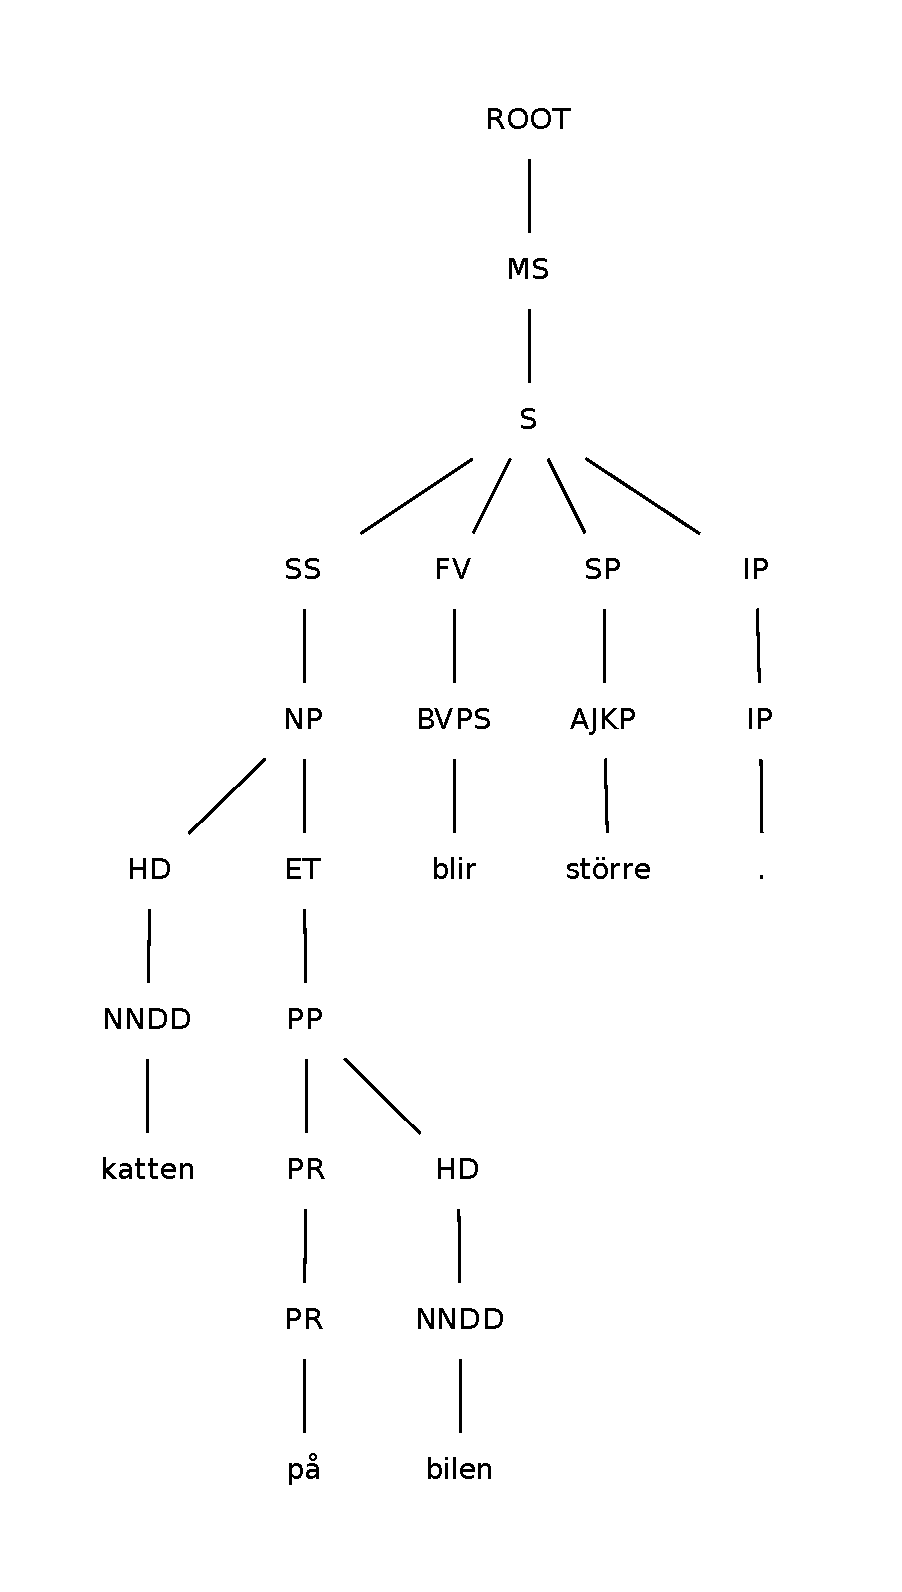
\includegraphics[width=130pt,height=200pt]{taltree.pdf}
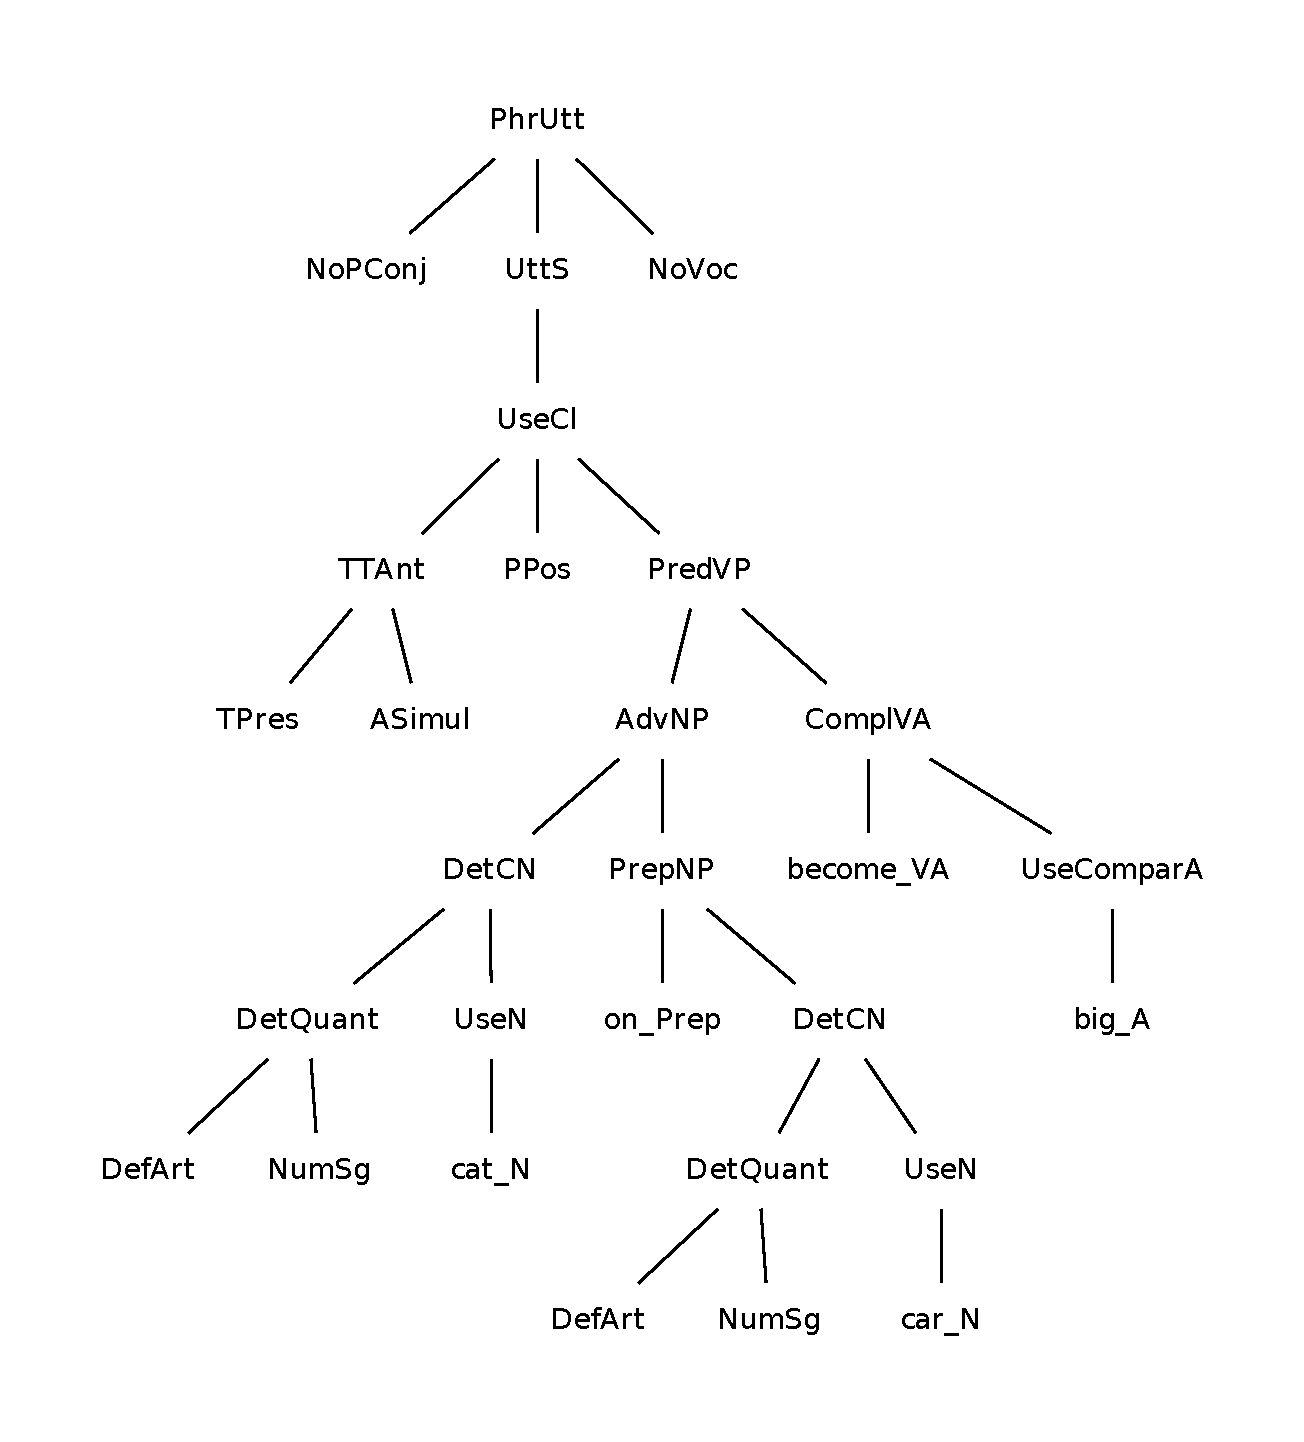
\includegraphics[width=170pt,height=200pt]{gftree.pdf}
\end{frame}

%\begin{frame}
%\frametitle{mapping}
%\framesubtitle{problems} 
%so far 42\% of the easy sentences are totally mapped 
%       10\% not at all
%
%avp
%differnt parsings
%\end{frame}
\begin{frame}

\frametitle{Mapping}
\framesubtitle{Benefits} 
\begin{itemize}
\item{Evaluate the parser}
\pause
\item{Identify grammatical constructions not current in the GF grammar}
\pause
\item{Enable good lexical extraction}
\pause
\item{Extract probabilities for GF functions}
\end{itemize}
% why it's hard (396 hur och hur)
%goals
\end{frame}


\begin{frame}
\frametitle{The grammar}
\framesubtitle{Current work} 
\begin{tabular}{ll}
\textbf{ReflGenVP} & VPSlash  $\rightarrow$ ReflCN $\rightarrow$ VP \\
& \emph{han ger sina små barn till dem} \\
% \\ but not \emph{sig själv}, \emph{han äter alla sina äpplen} or \emph{han ger sig till sig}  \\
  %relate to Peter - sig/sig själv, can't say hon ger sig till sig

\alert{\textbf{PassVP}}
  & \alert{V2 $\rightarrow$ VP} \\
& \alert{\emph{äpplet åts},}\alert{\emph{boken gavs till honom}} \\ 


\alert{\textbf{AdvVPSlash}} & \alert{VPSlash $\rightarrow$ Adv $\rightarrow$ VPSlash} \\
& \alert{\emph{hon åt redan äpplet}, \emph{hon är redan här}}\\

\alert{\textbf{PPartAP}} & \alert{V2 $\rightarrow$ AP} \\
& \alert{\emph{det är skrivet},\emph{den skrivna artikeln}}
\end{tabular}\\
  
\end{frame}

\begin{frame}[containsverbatim]
%% vad ska det heta???
\frametitle{Reflexive genitive verb phrase}
\framesubtitle{Problems} 
\begin{tabular}{ll}
Can say:&  \emph{han ger den till sin lilla katt} \\
 &        \emph{han ger sin egen katt till honom} \\
\end{tabular} \\
% fixa indentering
%\begin{tabular}{ll}
%\indent \small{\verb|ReflCN NumSg (AdjCN (PositA small_A) (UseN cat_N)))|} & \\
%\end{tabular} \\

\begin{tabular}{ll}
But can not say: & \emph{alla sina barn} \\
 & \emph{all sin undervisning} \\
 & \emph{han ger sina pengar till sina barn}
% & \emph{sin urgamla rätt att ...}\\  % N2V?
\end{tabular} \\
%hur löses det för vår? (inget problem för det hör ej ihop med subj)

\end{frame}


%kolla upp dessa i stort lexikon
\begin{frame}
 \renewcommand{\baselinestretch}{1.5}
\frametitle{The grammar}
\framesubtitle{Current work} 
\begin{tabular}{ll}
\alert{\textbf{ReflGenVP}} & \alert{VPSlash $\rightarrow$ ReflCN $\rightarrow$ VP} \\
& \alert{\emph{han ger sina små barn till dem}} \\
% \\ but not \emph{sig själv}, \emph{han äter alla sina äpplen} or \emph{han ger sig till sig}  \\
  %relate to Peter - sig/sig själv, can't say hon ger sig till sig
%
%%RelNP' "flickan, som inte ätit äpplen"
%% (RelNp "flickan , sådan att hon inte åt äpplen")
{\textbf{PassVP}} & V2 $\rightarrow$ VP \\%  (should be VPSlash $\rightarrow$ VP) \\
& \emph{äpplet åts} \\ % \;
 %\emph{("äpplet blev ätet")}\\ % boken gavs till honom


% CompAdv here, plus we need ComlVVAdv, Pass? osv
\alert{\textbf{AdvVPSlash}} & \alert{VPSlash $\rightarrow$ Adv $\rightarrow$ VPSlash} \\
& \alert{\emph{hon åt redan äpplet}, \emph{hon är redan här}}\\
% &\emph{("hon åt äpplet redan")} \\

\alert{\textbf{PPartAP}} & \alert{V2 $\rightarrow$ AP} \\
& \alert{\emph{det är skrivet},\emph{den skrivna artikeln}}
\end{tabular}\\
  
\end{frame}

\begin{frame}[containsverbatim]
\frametitle{Passive Form}
\framesubtitle{Problems} 
Only accepts verbs of type \verb|V2| \\
Cannot say \; \emph{Boken gavs till honom}\\
The type should be \verb|VPSlash -> VP|, but verb phrases does not carry
information about the passive form\\

\end{frame}

\begin{frame}
\frametitle{The grammar}
\framesubtitle{Current work} 
\begin{tabular}{ll}
\alert{\textbf{ReflGenVP}} & \alert{VPSlash $\rightarrow$ ReflCN $\rightarrow$ VP} \\
& \alert{\emph{han ger sina små barn till dem}} \\

 %\emph{("äpplet blev ätet")}\\ % boken gavs till honom
\alert{\textbf{PassVP}}
  & \alert{V2 $\rightarrow$ VP} \\ % (should be VPSlash $\rightarrow$ VP)} \\
& \alert{\emph{äpplet åts},}\alert{\emph{boken gavs till honom}} \\ 

% CompAdv here, plus we need ComlVVAdv, Pass? osv
\textbf{AdvVPSlash} & VPSlash $\rightarrow$ Adv $\rightarrow$ VPSlash \\
& \emph{hon åt redan äpplet}, \emph{hon är redan här}\\
% &\emph{("hon åt äpplet redan")} \\

\alert{\textbf{PPartAP}} & \alert{V2 $\rightarrow$ AP} \\
& \alert{\emph{det är skrivet},\emph{den skrivna artikeln}}
\end{tabular}\\
%list of functions
%examples
%difficulties
%sådan
\end{frame}

\begin{frame}
\frametitle{Adverbs describing VPSlash}
\framesubtitle{Example} 
\small{\textbf{AdvVPSlash}}\hspace{160pt}
\small{\textbf{AdvVP}}
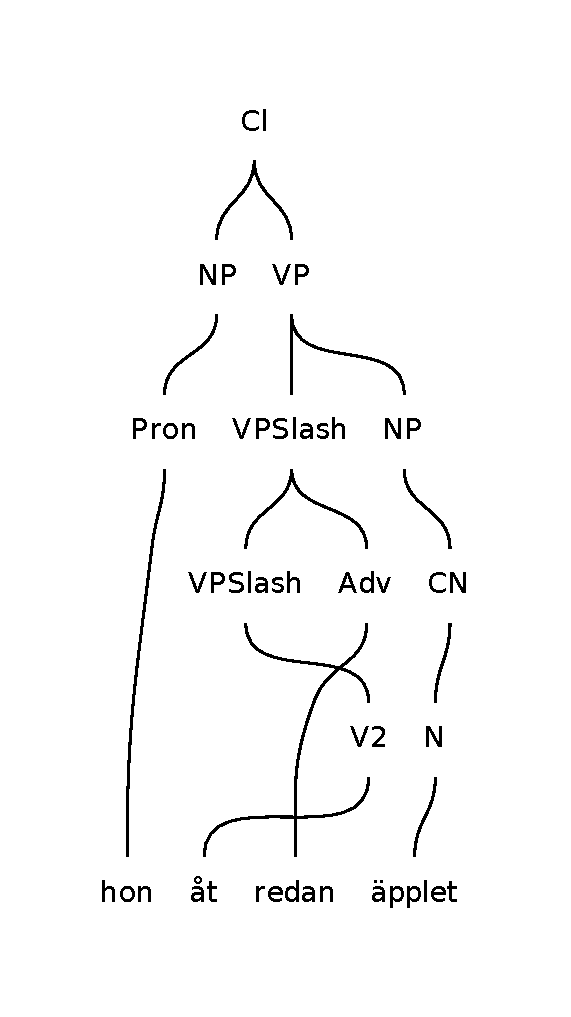
\includegraphics[width=170pt,height=200pt]{advVP.pdf}
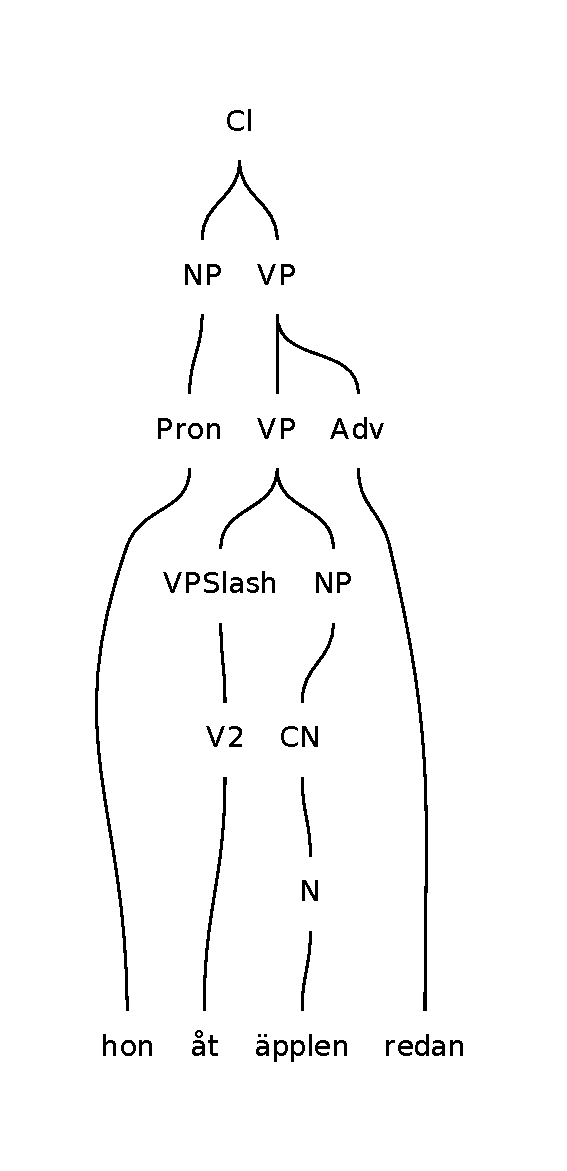
\includegraphics[width=170pt,height=200pt]{advVP2.pdf}
\end{frame}



\begin{frame}
\frametitle{The grammar}
\framesubtitle{Current work} 
\begin{tabular}{ll}
\alert{\textbf{ReflGenVP}} & \alert{VPSlash $\rightarrow$ ReflCN $\rightarrow$ VP} \\
& \alert{\emph{han ger sina små barn till dem}} \\

 %\emph{("äpplet blev ätet")}\\ % boken gavs till honom
\alert{\textbf{PassVP}}
  & \alert{V2 $\rightarrow$ VP} \\ % (should be VPSlash $\rightarrow$ VP)} \\
& \alert{\emph{äpplet åts},}\alert{\emph{boken gavs till honom}} \\ 

% CompAdv here, plus we need ComlVVAdv, Pass? osv
\alert{\textbf{AdvVPSlash}} & \alert{VPSlash $\rightarrow$ Adv $\rightarrow$ VPSlash} \\
& \alert{\emph{hon åt redan äpplet}, \emph{hon är redan här}}\\
% &\emph{("hon åt äpplet redan")} \\

\textbf{PPartAP} & V2 $\rightarrow$ AP \\
& \emph{det är skrivet},\emph{den skrivna artikeln}
\end{tabular}\\
\pause
%Easy sentences with known words (old testsuite) : 92 out of 118 (78\%) \\
%list of functions
%examples
%difficulties
%sådan
\end{frame}



\begin{frame}
 \renewcommand{\baselinestretch}{1.0}
\frametitle{Perfect Participle}
\framesubtitle{What type of functions do we need?} 
PPartAP cannot yet handle \emph{det är givet till henne} or \emph{de gågna åren} \\
% Adjective or verb? \\
%attribut- predikativ
\pause
Some examples:
\begin{itemize}
\item{ \textbf{V} \small{\emph{försvunnen}}, \small{\emph{slocknad}}}
\pause
\item{\textbf{V2 or V?} \small{\emph{en ökad effektiv information}},
\small{\emph{en minskad benägenhet}}} \\
\pause
\item{\textbf{V2}
\small{\emph{de stegrade hyrorna}},
\small{\emph{som aldrig är skalad}}, % (industriskalad, skalkokt)}} \\
\small{\emph{eftertraktade lägenheter}}} \\
\pause
\item{\textbf{V3} \small{\emph{de är skickade till mig}}}
\pause
\item{\textbf{VS} \small{\emph{han blev ombedd att gå}}}
\pause
\item{\textbf{Adj?}
\small{\emph{en fritt vuxen natur }},
\small{\emph{centralt belägna}},
\small{\emph{misstänkt }}}% \\% (av)}
\end{itemize}
\pause

VPSlash, V2, V?\\
%\emph{en kvalificerad majoritet} \\
%\emph{kokt potatis}} \\% (av)}
%& \emph{i en gången tids svenska bondesamhälle}  \\% 4872    
%?
%\emph{vår behandlade potatis} \\
%\emph{är oroad} \\
%\emph{beprövad}  \\ % (av)
%\emph{de levererar den doppad i askorbinsyra} 
\end{frame}

\begin{frame}
 \renewcommand{\baselinestretch}{1.0}
\frametitle{The Grammar}
\framesubtitle{Future work} 
Many words are treated differently in GF and Talbanken. \\
\begin{tabular}{lll}
& \textbf{Talbanken} & \textbf{GF} \\
\emph{mycket} & Pronoun, adverb &  Determiner and adverb\\
& &\emph{mycket blir bättre}, \emph{hon äter mycket}\\
\pause
\emph{bara} & Adverb & Predeterminer and AdV \\ %% nice name here!!
& &\emph{bara barn är små}, \emph{hon bara log}, \emph{hon log bara} \\
\end{tabular} \\
\vspace{0.5cm}
\pause
Pronouns in Talbanken:
\emph{fler},\emph{båda}\\
   \emph{det finns fler upplysningar}, \emph{fler är där}, \emph{analfabeterna blir fler} %sådana
\end{frame}

\begin{frame}
 \renewcommand{\baselinestretch}{1.0}
\frametitle{The Grammar}
\framesubtitle{Future work} 
\begin{itemize}
\item{Reciprocal pronouns - \emph{varandra }}
\pause
\item{\emph{Slags, sorts}: \emph{en sort\textbf{s} katt}, \emph{katter av en sort}}
\pause
\item{\emph{Den yngsta    är gladast}}
\pause
\item{\emph{De  arbetande är tröttast}}
\pause
\item{Idioms, AVP (adverb phrases)\\
\emph{till exempel, i stället,i fortsättningen}}
%\item{\emph{minst}, \emph{lika}}
\end{itemize}
\end{frame}

\begin{frame}
\frametitle{Goals}
\framesubtitle{Goals for Christmas} 
\begin{itemize}
\item{Finish and evaluate mapping}
\pause
\item{Extend grammar}
\pause
\item{Evaluation}
\pause
\item{New mapping of SALDO - making it easy to keep up-to-date}
\pause
\item{?}
\end{itemize}
\end{frame}

\begin{frame}
    \frametitle{The end}
\large\begin{center}Thanks for listening\end{center}
\end{frame}
\end{document}

